% $Header: /projects/VU-SAGA/Papers/saga_engine_2006/generaldesign.tex,v 1.9 2006/08/13 18:01:00 hkaiser Exp $

The implementation level requirements to the SAGA reference
implementation as described in the previous section are directly
motivating a number of design objectives. Our most important objective was to 
design a state-of-the-art Grid application framework satisfying the majority 
of user-needs while staying as flexible as possible. 

So it is obvious that this flexibility and extensibility of the implementation, 
in multiple dimensions, is a central point in the design, and in fact dominates
the overall architecture of the library (see figure~\ref{fig:archi}).  As
a summary: only components known to be stable, such as the SAGA
look\,\&\,feel and the SAGA utility classes, are statically included
in the library -- all other aspects of the API implementation, such as
the core SAGA classes and the middleware compile time and run time
bindings, are designed to be components which can be added and
selected separately.

\begin{figure}[!ht]
 \begin{center}
  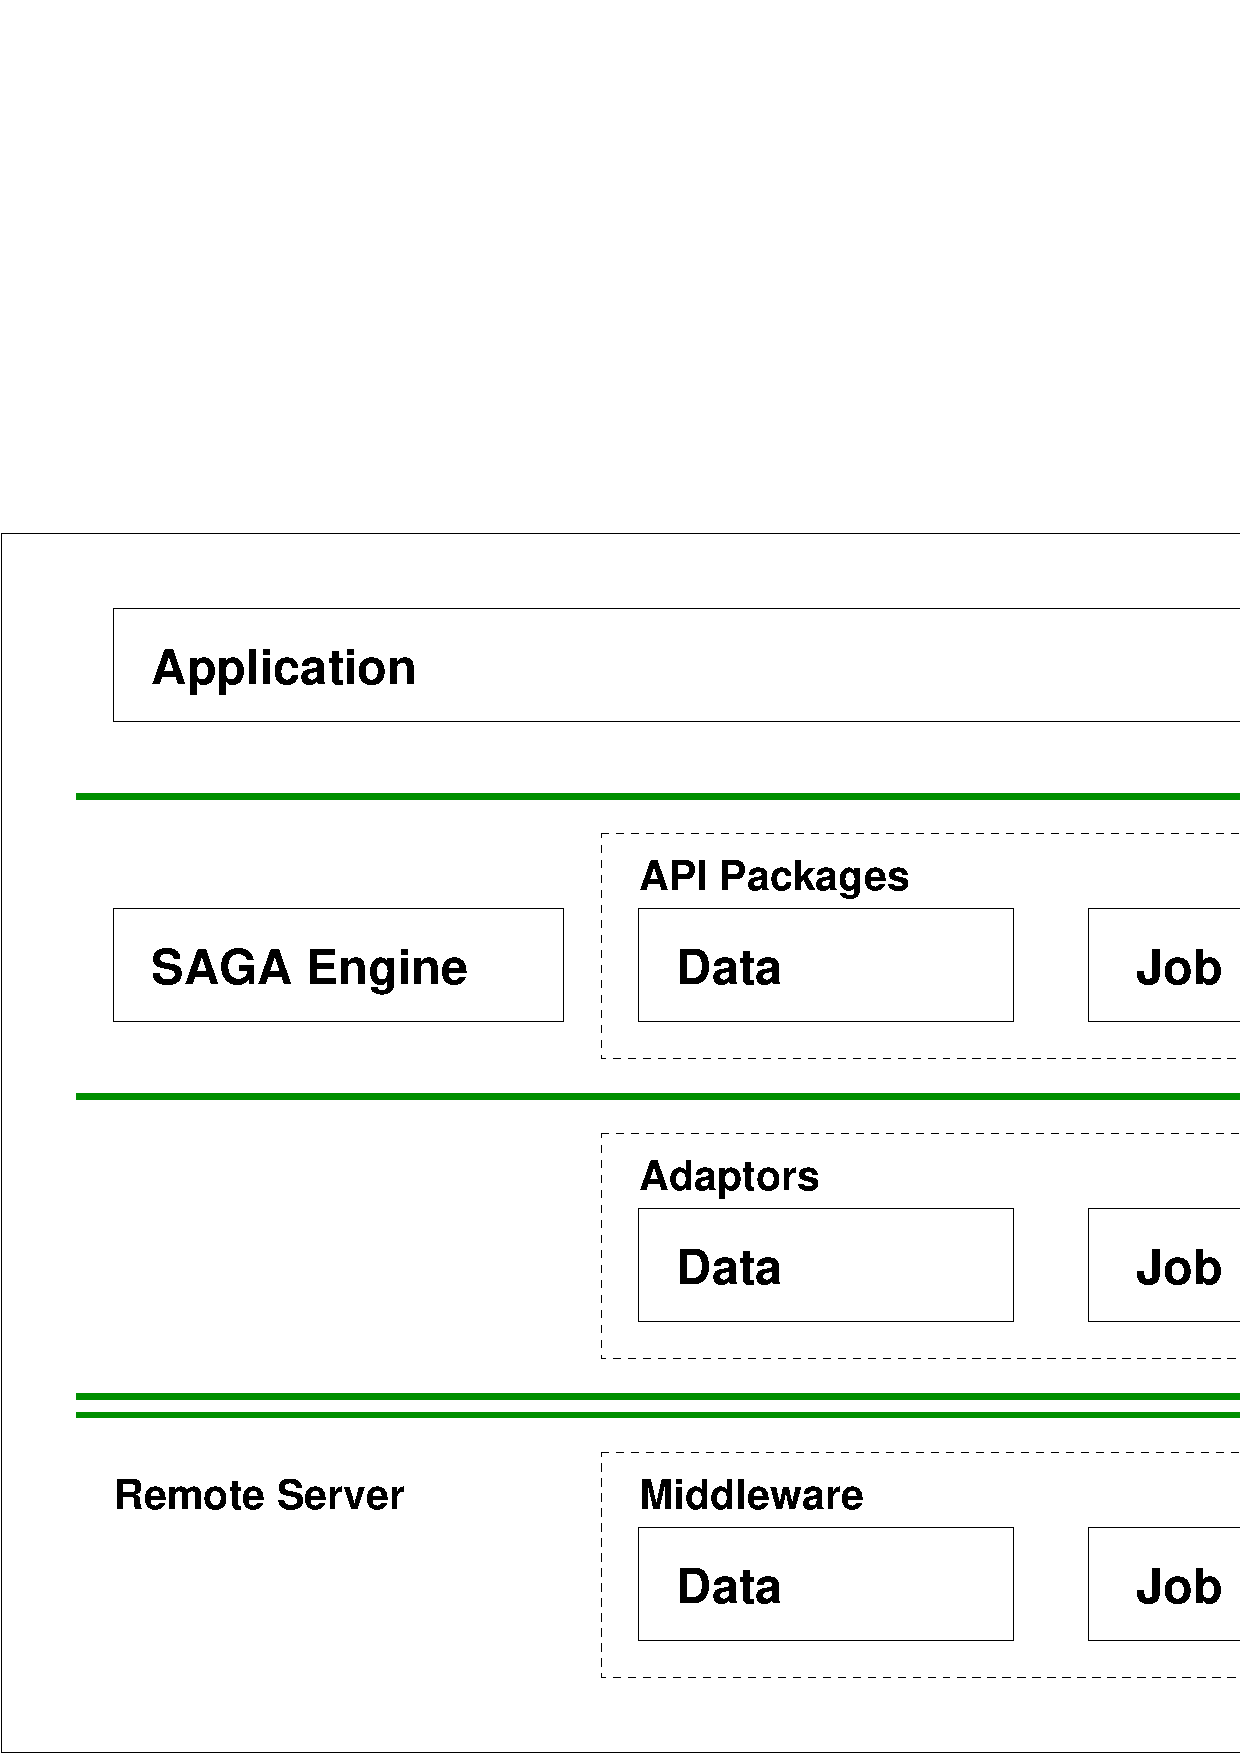
\includegraphics[width=0.47\textwidth]{images/saga_architecture}
  \caption{\label{fig:archi}
    Architecture: A lightweight engine dispatches SAGA 
    calls do dynamically loaded middleware adaptors.}
 \end{center}
\end{figure}

\subsection{Design Objectives}

	The Simple API for Grid Applications is, by definition, well ... \I{simple}. 
	This doesn't imply the implementation itself has to be simple. We made a major 
	effort to build	as much logic and functionality as possible into the 
	SAGA engine providing all the needed common functionality. This	enables the 
	user to extend it with minimal effort. On the other hand, 
	the library \I{is} designed to be easy to build, use, and deploy. 
	
	As described in the previous section, a SAGA implementation has to cope 
	with a multitude of different dynamic boundary conditions. A major design
	objective therefore was to maximize decoupling of different components
	of the developed library to allow for as much as possible \I{flexibility}, 
	\I{adaptability} and \I{modularity}.

	As the SAGA implementation is expected to be used on different platforms
	and operating systems we strive for maximal implementation \I{portability}. 

  The API should be \I{extensible} with minimal effort: ideally,
  adding a new API class is orthogonal to all other properties of the
  implementation, and immediately benefits from those.


\subsection{The Overall Architecture}

	To meet these goals we decided to decouple the library components
	in three dimensions. These three dimensions are completely orthogonal -- 
	the user of the library may use and combine these at free will and may 
	develop additional suitable components usable in tight integration with 
	the provided modules.

\subsubsection{Horizontal Extensibility -- API Packages}
\label{ssec:apipackages}

	The SAGA specification is object oriented and defines a set of API groups
	keeping objects of related functionality together (packages). Our implementation
	uses this functional grouping to define \I{API packages}.	The currently 
	defined packages are: file management, job management, remote procedure calls, 
  replica management, and data streaming. Each of 
	these packages constitutes a separate and independent module. 
	These modules depend only on the SAGA engine, the user is therefore free to 
	use and link only those modules actually needed by the application, minimizing 
	the memory footprint.
	
	New API packages are expected to be added in the future as the SAGA specification
	evolves. It is straightforward to add new packages since all common operations 
	needed inside these packages (as adaptor loading and selection, and method call routing) 
	are imported from the SAGA engine.  The creation of new packages is
  essentially reduced to:

  \begin{shortlist}
	   \item add the API (5) package files, and declare the classes,
	   \item reflect the SAGA object hierarchy (more details below, in
	   			 section~\ref{ssec:pimpl}), 
	   \item add class methods
  \end{shortlist}

  The declaration and definition of the API methods is greatly simplified by
  several macros, which essentially correspond directly to the methods
  SIDL specification.  We consider to (partly) automate the generation
  of new packages, by parsing the SIDL specification and generating the
  class stubs and class method specifications.  The user must then
  only add the required include files to get a full fledged,
  compilable and usable SAGA API implementation package. This approach will 
  allow us to generate other SAGA language bindings from the SIDL 
  specification as well, such as for the C and FORTRAN languages.
  
  Additionally we are using the Boost.Wave~\cite{wave_website} C++ preprocessor 
  and special \#pragma's implemented by this tool to pre-generate 
  partially macro expanded sources allowing to overcome the disadvantages 
	of plain macros, hence simplifying debugging and improving readability.
  
  % I have a perl script which does the essential part of that
  % generation process already - I stopped maintaining it as we
  % updated the packages, but will get it up to date at some point.  I
  % could actually create the old package types, only the inheritance
  % stuff and the impl initialization was missing :-) -- AM
	
\subsubsection{Vertical Extensibility -- Middleware Bindings}

	A layered architecture (see figure~\ref{fig:archi}) allows us to vertically decouple the SAGA 
	API from the used middleware. Separate adaptors, either loaded at 
	runtime, or pre-bound at link time, dispatch the different API
	function calls to the appropriate middleware. Most of the time
	there will be a separate set of adaptors for each type of middleware to 
	support. These adaptors implement a well defined capability provider
	interface (CPI) and expose that to the top layer of the library, which makes it
	possible to switch adaptors at runtime and hence to switch between 
	different (and even concurrent) middleware services providing the requested 
	functionality. The top library layer dispatches the API function calls 
	to the corresponding CPI function.
	
	The top library layer additionally contains the \I{SAGA engine} module,
  which implements:
	\begin{shortlist}
		\item core SAGA objects such as session, context, task or 
					task\_container -- these objects are responsible for the
          SAGA look\,\&\,feel, and are needed by all API packages;
		\item common functions needed to load and select matching 
					adaptors, to perform generic call routing from API 
					functions to the selected adaptor, to provide necessary
					fall back implementations for the synchronous and asynchronous
					variants of the API functions (if these are not supported by
          the selected adaptor).
	\end{shortlist}

	The dynamic nature of this layered architecture enables easy future 
	extensions by adding new adaptors, coping with emerging grid standards 
	and new or changed grid middleware.
	

\subsubsection{Extensibility for Optimization and Features} 

  Many features of the engine module are implemented by intercepting,
  analyzing, managing, and rerouting function calls between the API packages,
  where they get issued, and the adaptors, where they get executed
  and forwarded to the middleware.  To generalize that management
  layer, a PIMPL~\cite{pimpl} (Private Implementation) 
  idiom was chosen, and is rigorously
  used throughout the SAGA implementation.  That PIMPL layering allows
  for a number of additional properties to be transparently
  implemented, and experimen\-ted with, without any reflected change in
  either the API packages nor in the adaptor layers.  These features
  include:

	\begin{shortlist}
    \item generic call routing
	  \item task monitoring and optimization
    \item security management
    \item late binding
	  \item fallback on adaptor invocation errors
    \item latency hiding mechanisms
	\end{shortlist}

	The decoupling of these features from the API and 
  the adaptors succeeds, essentially, because these properties 
  affect only the IMPL side of the PIMPL layers.  

  Firstly, the private implementation classes all inherit from the same
  base class -- only that base class is handled in the central engine
  module, so the engine can automatically cope with new API packages
  and adaptors.  Secondly, all method calls are also handled
  generically in the engine.
  
  The engine module is hence fully generic, and loosely coupled to
  both the API and the adaptor layers.  Any changes to the engine, all
  optimization, latency hiding techniques, monitoring features etc.
  can be implemented in the engine generically, and are orthogonal to
  the API and adaptor extensions.  Hence, the extensibility of the
  engine represents the third orthogonal axis in the libraries
  extensibility scheme.

  % This is now described in 4.1.2 -- AM
  % 
	% Any of the package API functions are exposed in three variants: synchronous
	% asynchronous ans task based execution. The synchronous variant blocks
	% while the requested function is executed. On the other hand the asynchronous 
	% and task based variants immediately return a task instance encapsulating
	% the requested function call, whereas the task returned from the asynchronous 
	% call has already been star\-ted. The task returned from the task based 
	% function call needs to be started explicitely by calling the task::run() 
	% member.

